\documentclass[twoside]{book}

% Packages required by doxygen
\usepackage{fixltx2e}
\usepackage{calc}
\usepackage{doxygen}
\usepackage[export]{adjustbox} % also loads graphicx
\usepackage{graphicx}
\usepackage[utf8]{inputenc}
\usepackage{makeidx}
\usepackage{multicol}
\usepackage{multirow}
\PassOptionsToPackage{warn}{textcomp}
\usepackage{textcomp}
\usepackage[nointegrals]{wasysym}
\usepackage[table]{xcolor}

% Font selection
\usepackage[T1]{fontenc}
\usepackage[scaled=.90]{helvet}
\usepackage{courier}
\usepackage{amssymb}
\usepackage{sectsty}
\renewcommand{\familydefault}{\sfdefault}
\allsectionsfont{%
  \fontseries{bc}\selectfont%
  \color{darkgray}%
}
\renewcommand{\DoxyLabelFont}{%
  \fontseries{bc}\selectfont%
  \color{darkgray}%
}
\newcommand{\+}{\discretionary{\mbox{\scriptsize$\hookleftarrow$}}{}{}}

% Page & text layout
\usepackage{geometry}
\geometry{%
  a4paper,%
  top=2.5cm,%
  bottom=2.5cm,%
  left=2.5cm,%
  right=2.5cm%
}
\tolerance=750
\hfuzz=15pt
\hbadness=750
\setlength{\emergencystretch}{15pt}
\setlength{\parindent}{0cm}
\setlength{\parskip}{3ex plus 2ex minus 2ex}
\makeatletter
\renewcommand{\paragraph}{%
  \@startsection{paragraph}{4}{0ex}{-1.0ex}{1.0ex}{%
    \normalfont\normalsize\bfseries\SS@parafont%
  }%
}
\renewcommand{\subparagraph}{%
  \@startsection{subparagraph}{5}{0ex}{-1.0ex}{1.0ex}{%
    \normalfont\normalsize\bfseries\SS@subparafont%
  }%
}
\makeatother

% Headers & footers
\usepackage{fancyhdr}
\pagestyle{fancyplain}
\fancyhead[LE]{\fancyplain{}{\bfseries\thepage}}
\fancyhead[CE]{\fancyplain{}{}}
\fancyhead[RE]{\fancyplain{}{\bfseries\leftmark}}
\fancyhead[LO]{\fancyplain{}{\bfseries\rightmark}}
\fancyhead[CO]{\fancyplain{}{}}
\fancyhead[RO]{\fancyplain{}{\bfseries\thepage}}
\fancyfoot[LE]{\fancyplain{}{}}
\fancyfoot[CE]{\fancyplain{}{}}
\fancyfoot[RE]{\fancyplain{}{\bfseries\scriptsize Generated by Doxygen }}
\fancyfoot[LO]{\fancyplain{}{\bfseries\scriptsize Generated by Doxygen }}
\fancyfoot[CO]{\fancyplain{}{}}
\fancyfoot[RO]{\fancyplain{}{}}
\renewcommand{\footrulewidth}{0.4pt}
\renewcommand{\chaptermark}[1]{%
  \markboth{#1}{}%
}
\renewcommand{\sectionmark}[1]{%
  \markright{\thesection\ #1}%
}

% Indices & bibliography
\usepackage{natbib}
\usepackage[titles]{tocloft}
\setcounter{tocdepth}{3}
\setcounter{secnumdepth}{5}
\makeindex

% Hyperlinks (required, but should be loaded last)
\usepackage{ifpdf}
\ifpdf
  \usepackage[pdftex,pagebackref=true]{hyperref}
\else
  \usepackage[ps2pdf,pagebackref=true]{hyperref}
\fi
\hypersetup{%
  colorlinks=true,%
  linkcolor=blue,%
  citecolor=blue,%
  unicode%
}

% Custom commands
\newcommand{\clearemptydoublepage}{%
  \newpage{\pagestyle{empty}\cleardoublepage}%
}

\usepackage{caption}
\captionsetup{labelsep=space,justification=centering,font={bf},singlelinecheck=off,skip=4pt,position=top}

%===== C O N T E N T S =====

\begin{document}

% Titlepage & ToC
\hypersetup{pageanchor=false,
             bookmarksnumbered=true,
             pdfencoding=unicode
            }
\pagenumbering{alph}
\begin{titlepage}
\vspace*{7cm}
\begin{center}%
{\Large F\+I\+G\+U\+R\+E-\/project }\\
\vspace*{1cm}
{\large Generated by Doxygen 1.8.13}\\
\end{center}
\end{titlepage}
\clearemptydoublepage
\pagenumbering{roman}
\tableofcontents
\clearemptydoublepage
\pagenumbering{arabic}
\hypersetup{pageanchor=true}

%--- Begin generated contents ---
\chapter{Hierarchical Index}
\section{Class Hierarchy}
This inheritance list is sorted roughly, but not completely, alphabetically\+:\begin{DoxyCompactList}
\item \contentsline{section}{figure}{\pageref{classfigure}}{}
\begin{DoxyCompactList}
\item \contentsline{section}{disque}{\pageref{classdisque}}{}
\item \contentsline{section}{rectangle}{\pageref{classrectangle}}{}
\item \contentsline{section}{triangle}{\pageref{classtriangle}}{}
\end{DoxyCompactList}
\end{DoxyCompactList}

\chapter{Class Index}
\section{Class List}
Here are the classes, structs, unions and interfaces with brief descriptions\+:\begin{DoxyCompactList}
\item\contentsline{section}{\hyperlink{classdisque}{disque} \\*Classe de definition d\textquotesingle{}une figure disque }{\pageref{classdisque}}{}
\item\contentsline{section}{\hyperlink{classfigure}{figure} }{\pageref{classfigure}}{}
\item\contentsline{section}{\hyperlink{classrectangle}{rectangle} }{\pageref{classrectangle}}{}
\item\contentsline{section}{\hyperlink{classtriangle}{triangle} }{\pageref{classtriangle}}{}
\end{DoxyCompactList}

\chapter{File Index}
\section{File List}
Here is a list of all documented files with brief descriptions\+:\begin{DoxyCompactList}
\item\contentsline{section}{/home/epsi/figure/figure/src/\hyperlink{disque_8h}{disque.\+h} \\*Fichier de la classe disque }{\pageref{disque_8h}}{}
\item\contentsline{section}{/home/epsi/figure/figure/src/\hyperlink{figure_8h}{figure.\+h} \\*Définition de la classe parent \char`\"{}figure\char`\"{} }{\pageref{figure_8h}}{}
\item\contentsline{section}{/home/epsi/figure/figure/src/\hyperlink{rectangle_8h}{rectangle.\+h} \\*Définition de la classe rectangle }{\pageref{rectangle_8h}}{}
\item\contentsline{section}{/home/epsi/figure/figure/src/{\bfseries triangle.\+h} }{\pageref{triangle_8h}}{}
\end{DoxyCompactList}

\chapter{Class Documentation}
\hypertarget{classdisque}{}\section{disque Class Reference}
\label{classdisque}\index{disque@{disque}}


classe de definition d\textquotesingle{}une figure disque  




{\ttfamily \#include $<$disque.\+h$>$}



Inheritance diagram for disque\+:
\nopagebreak
\begin{figure}[H]
\begin{center}
\leavevmode
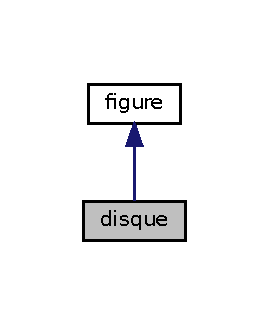
\includegraphics[width=129pt]{classdisque__inherit__graph}
\end{center}
\end{figure}


Collaboration diagram for disque\+:
\nopagebreak
\begin{figure}[H]
\begin{center}
\leavevmode
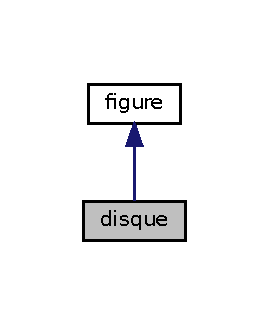
\includegraphics[width=129pt]{classdisque__coll__graph}
\end{center}
\end{figure}
\subsection*{Public Member Functions}
\begin{DoxyCompactItemize}
\item 
\mbox{\Hypertarget{classdisque_a0b2efca226d978af39559a696bb84488}\label{classdisque_a0b2efca226d978af39559a696bb84488}} 
void {\bfseries set\+Rayon} (int A)
\item 
\mbox{\Hypertarget{classdisque_a6503c0a336e4391d4a0254b5d720d029}\label{classdisque_a6503c0a336e4391d4a0254b5d720d029}} 
float {\bfseries get\+Perimetre} () override
\item 
\mbox{\Hypertarget{classdisque_aafffe3cc0969974593133322b8d12719}\label{classdisque_aafffe3cc0969974593133322b8d12719}} 
float {\bfseries get\+Surface} () override
\end{DoxyCompactItemize}
\subsection*{Public Attributes}
\begin{DoxyCompactItemize}
\item 
\mbox{\Hypertarget{classdisque_ac9ae86ee1309e5fec237632aeb70c0af}\label{classdisque_ac9ae86ee1309e5fec237632aeb70c0af}} 
float {\bfseries rayon}
\end{DoxyCompactItemize}


\subsection{Detailed Description}
classe de definition d\textquotesingle{}une figure disque 

utilisation du rayon en entrée pour renvoyer le perimetre et la surface 

The documentation for this class was generated from the following files\+:\begin{DoxyCompactItemize}
\item 
/home/epsi/figure/figure/src/\hyperlink{disque_8h}{disque.\+h}\item 
/home/epsi/figure/figure/src/disque.\+cpp\end{DoxyCompactItemize}

\hypertarget{classfigure}{}\section{figure Class Reference}
\label{classfigure}\index{figure@{figure}}


Inheritance diagram for figure\+:
\nopagebreak
\begin{figure}[H]
\begin{center}
\leavevmode
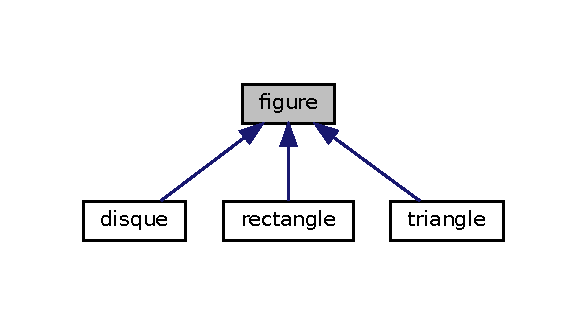
\includegraphics[width=282pt]{classfigure__inherit__graph}
\end{center}
\end{figure}
\subsection*{Public Member Functions}
\begin{DoxyCompactItemize}
\item 
\mbox{\Hypertarget{classfigure_ad1cc1bebf09fcfcf96490934895d1478}\label{classfigure_ad1cc1bebf09fcfcf96490934895d1478}} 
virtual float {\bfseries get\+Perimetre} ()=0
\item 
\mbox{\Hypertarget{classfigure_ae0301c7790ae10bdce44f034ac825cb4}\label{classfigure_ae0301c7790ae10bdce44f034ac825cb4}} 
virtual float {\bfseries get\+Surface} ()=0
\end{DoxyCompactItemize}


The documentation for this class was generated from the following files\+:\begin{DoxyCompactItemize}
\item 
/home/epsi/figure/figure/src/\hyperlink{figure_8h}{figure.\+h}\item 
/home/epsi/figure/figure/src/figure.\+cpp\end{DoxyCompactItemize}

\hypertarget{classrectangle}{}\section{rectangle Class Reference}
\label{classrectangle}\index{rectangle@{rectangle}}


Inheritance diagram for rectangle\+:
\nopagebreak
\begin{figure}[H]
\begin{center}
\leavevmode
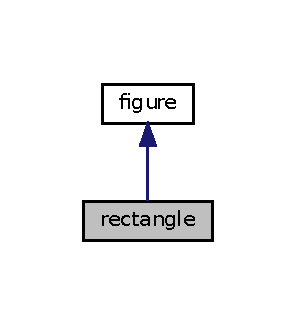
\includegraphics[width=142pt]{classrectangle__inherit__graph}
\end{center}
\end{figure}


Collaboration diagram for rectangle\+:
\nopagebreak
\begin{figure}[H]
\begin{center}
\leavevmode
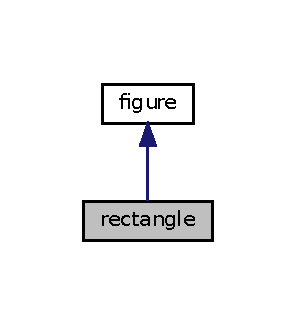
\includegraphics[width=142pt]{classrectangle__coll__graph}
\end{center}
\end{figure}
\subsection*{Public Member Functions}
\begin{DoxyCompactItemize}
\item 
\mbox{\Hypertarget{classrectangle_a7b8105e029fcfbd0bf8a99f91df2a4ed}\label{classrectangle_a7b8105e029fcfbd0bf8a99f91df2a4ed}} 
float {\bfseries get\+Perimetre} () override
\item 
\mbox{\Hypertarget{classrectangle_ae08cdfb566b44227e2aaf4e08671d60e}\label{classrectangle_ae08cdfb566b44227e2aaf4e08671d60e}} 
float {\bfseries get\+Surface} () override
\item 
\mbox{\Hypertarget{classrectangle_abdf1a061e88226c424173a2022234d9b}\label{classrectangle_abdf1a061e88226c424173a2022234d9b}} 
void {\bfseries Setlongueur} (float l)
\item 
\mbox{\Hypertarget{classrectangle_a179b4c863a4a47cbb4e5607124947124}\label{classrectangle_a179b4c863a4a47cbb4e5607124947124}} 
void {\bfseries Setlargeur} (float L)
\end{DoxyCompactItemize}
\subsection*{Public Attributes}
\begin{DoxyCompactItemize}
\item 
\mbox{\Hypertarget{classrectangle_a323614223c090cf3701e0877ff552328}\label{classrectangle_a323614223c090cf3701e0877ff552328}} 
float {\bfseries longueur}
\item 
\mbox{\Hypertarget{classrectangle_afcdec92029cdbf85d33d8e11f389b37e}\label{classrectangle_afcdec92029cdbf85d33d8e11f389b37e}} 
float {\bfseries largeur}
\end{DoxyCompactItemize}


The documentation for this class was generated from the following files\+:\begin{DoxyCompactItemize}
\item 
/home/epsi/figure/figure/src/\hyperlink{rectangle_8h}{rectangle.\+h}\item 
/home/epsi/figure/figure/src/rectangle.\+cpp\end{DoxyCompactItemize}

\hypertarget{classtriangle}{}\section{triangle Class Reference}
\label{classtriangle}\index{triangle@{triangle}}


Inheritance diagram for triangle\+:
\nopagebreak
\begin{figure}[H]
\begin{center}
\leavevmode
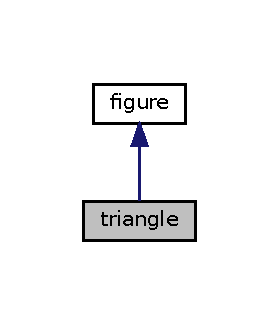
\includegraphics[width=134pt]{classtriangle__inherit__graph}
\end{center}
\end{figure}


Collaboration diagram for triangle\+:
\nopagebreak
\begin{figure}[H]
\begin{center}
\leavevmode
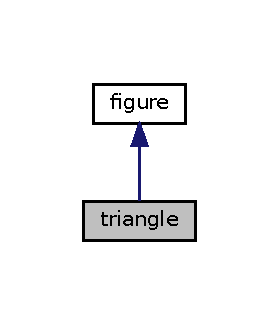
\includegraphics[width=134pt]{classtriangle__coll__graph}
\end{center}
\end{figure}
\subsection*{Public Member Functions}
\begin{DoxyCompactItemize}
\item 
\mbox{\Hypertarget{classtriangle_a972fd35b7e835e551bc70cb41e17b509}\label{classtriangle_a972fd35b7e835e551bc70cb41e17b509}} 
void {\bfseries Setcotes} (int a, int b, int c)
\item 
\mbox{\Hypertarget{classtriangle_ac768fd572b720d004150e6c71bf2071c}\label{classtriangle_ac768fd572b720d004150e6c71bf2071c}} 
float {\bfseries get\+Perimetre} () override
\item 
\mbox{\Hypertarget{classtriangle_a3726b59fd5c556403471d1813632b09a}\label{classtriangle_a3726b59fd5c556403471d1813632b09a}} 
float {\bfseries get\+Surface} () override
\end{DoxyCompactItemize}
\subsection*{Public Attributes}
\begin{DoxyCompactItemize}
\item 
\mbox{\Hypertarget{classtriangle_a9ed10544b194df91065464230384aaaf}\label{classtriangle_a9ed10544b194df91065464230384aaaf}} 
float {\bfseries basebc}
\item 
\mbox{\Hypertarget{classtriangle_ae42cf8cc51203613bb6e2f6d5628763c}\label{classtriangle_ae42cf8cc51203613bb6e2f6d5628763c}} 
float {\bfseries hauteur}
\item 
\mbox{\Hypertarget{classtriangle_a61b7d49c873cb8d4cabdde86c3fc66bf}\label{classtriangle_a61b7d49c873cb8d4cabdde86c3fc66bf}} 
float {\bfseries ab}
\item 
\mbox{\Hypertarget{classtriangle_abdee7cb1c7db557c13bfd0f7791fcdcc}\label{classtriangle_abdee7cb1c7db557c13bfd0f7791fcdcc}} 
float {\bfseries ac}
\end{DoxyCompactItemize}


The documentation for this class was generated from the following files\+:\begin{DoxyCompactItemize}
\item 
/home/epsi/figure/figure/src/triangle.\+h\item 
/home/epsi/figure/figure/src/triangle.\+cpp\end{DoxyCompactItemize}

\chapter{File Documentation}
\hypertarget{disque_8h}{}\section{/home/epsi/figure/figure/src/disque.h File Reference}
\label{disque_8h}\index{/home/epsi/figure/figure/src/disque.\+h@{/home/epsi/figure/figure/src/disque.\+h}}


fichier de la classe disque  


{\ttfamily \#include \char`\"{}figure.\+h\char`\"{}}\newline
Include dependency graph for disque.\+h\+:
\nopagebreak
\begin{figure}[H]
\begin{center}
\leavevmode
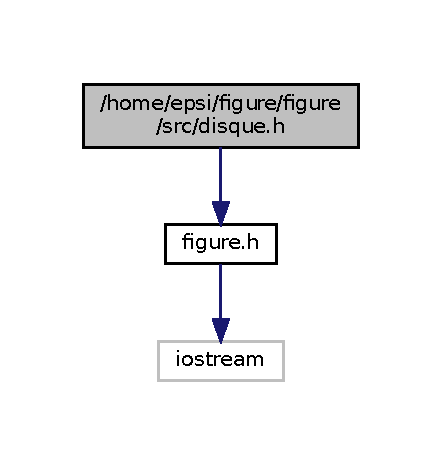
\includegraphics[width=212pt]{disque_8h__incl}
\end{center}
\end{figure}
\subsection*{Classes}
\begin{DoxyCompactItemize}
\item 
class \hyperlink{classdisque}{disque}
\begin{DoxyCompactList}\small\item\em classe de definition d\textquotesingle{}une figure disque \end{DoxyCompactList}\end{DoxyCompactItemize}


\subsection{Detailed Description}
fichier de la classe disque 

\begin{DoxyAuthor}{Author}
lucas 
\end{DoxyAuthor}

\hypertarget{figure_8h}{}\section{/home/epsi/figure/figure/src/figure.h File Reference}
\label{figure_8h}\index{/home/epsi/figure/figure/src/figure.\+h@{/home/epsi/figure/figure/src/figure.\+h}}


définition de la classe parent \char`\"{}figure\char`\"{}  


{\ttfamily \#include $<$iostream$>$}\newline
Include dependency graph for figure.\+h\+:
\nopagebreak
\begin{figure}[H]
\begin{center}
\leavevmode
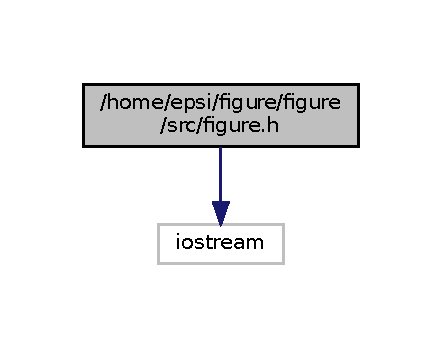
\includegraphics[width=212pt]{figure_8h__incl}
\end{center}
\end{figure}
This graph shows which files directly or indirectly include this file\+:
\nopagebreak
\begin{figure}[H]
\begin{center}
\leavevmode
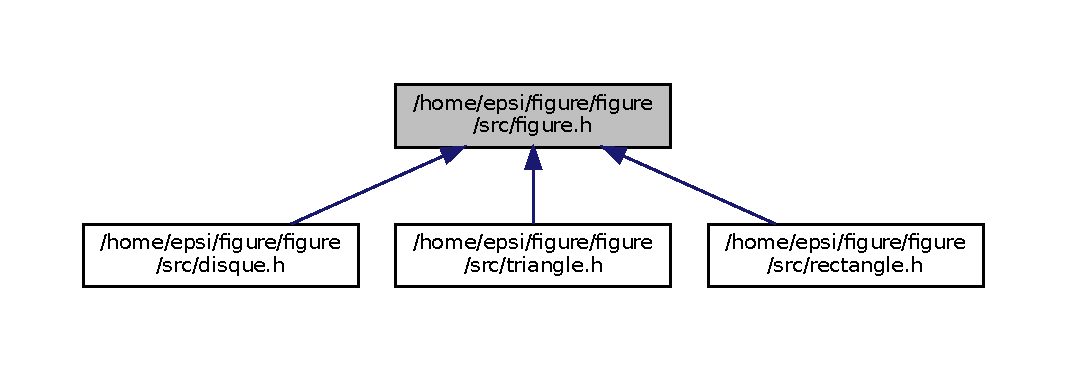
\includegraphics[width=350pt]{figure_8h__dep__incl}
\end{center}
\end{figure}
\subsection*{Classes}
\begin{DoxyCompactItemize}
\item 
class \hyperlink{classfigure}{figure}
\end{DoxyCompactItemize}


\subsection{Detailed Description}
définition de la classe parent \char`\"{}figure\char`\"{} 

\begin{DoxyAuthor}{Author}
lucas 
\end{DoxyAuthor}
\begin{DoxyVersion}{Version}
1.\+0 
\end{DoxyVersion}

\hypertarget{rectangle_8h}{}\section{/home/epsi/figure/figure/src/rectangle.h File Reference}
\label{rectangle_8h}\index{/home/epsi/figure/figure/src/rectangle.\+h@{/home/epsi/figure/figure/src/rectangle.\+h}}


définition de la classe rectangle  


{\ttfamily \#include \char`\"{}figure.\+h\char`\"{}}\newline
Include dependency graph for rectangle.\+h\+:
\nopagebreak
\begin{figure}[H]
\begin{center}
\leavevmode
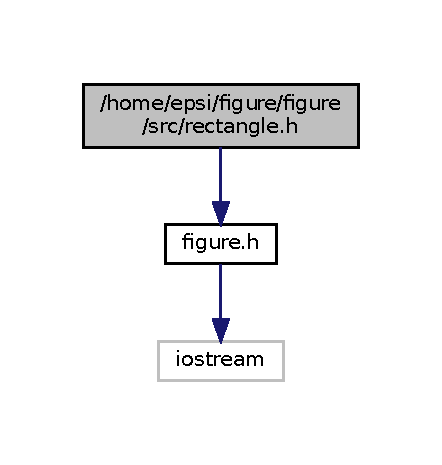
\includegraphics[width=212pt]{rectangle_8h__incl}
\end{center}
\end{figure}
\subsection*{Classes}
\begin{DoxyCompactItemize}
\item 
class \hyperlink{classrectangle}{rectangle}
\end{DoxyCompactItemize}


\subsection{Detailed Description}
définition de la classe rectangle 

\begin{DoxyAuthor}{Author}
lucas 
\end{DoxyAuthor}
\begin{DoxyVersion}{Version}
1.\+0 
\end{DoxyVersion}

%--- End generated contents ---

% Index
\backmatter
\newpage
\phantomsection
\clearemptydoublepage
\addcontentsline{toc}{chapter}{Index}
\printindex

\end{document}
